\documentclass[12pt letterpaper]{article}

\usepackage{fullpage}
\usepackage{graphicx}
\usepackage{amsmath}

\providecommand{\e}[1]{\ensuremath{\times 10^{#1}}}
\usepackage{gensymb}

\usepackage{float}


\title{Electron Beam Diffraction / Debye-Scherrer Diffraction at Graphite}
\author{Johnny Minor \\ Partner: Kayla Mitchell}
\date{\today}

\begin{document}

\maketitle

%abstract should have a very brief overiew of the goals and main results of the experiment. 
\begin{abstract}
In this experiment we studied the wave nature of electrons. In 1924 Louis de Broglie proposed that not only light have a particle-wave duality, but that also matter could exhibit a particle-wave duality. One of the first experiments to highlight this fact was Davidson and Germer's experiment where they aimed an electron beam at a nickel crystal and they saw the resulting diffraction pattern. Thus proving that electrons can exhibit a wave-like nature. In our experiment we aim an electron beam of 5.0 keV at a graphite powder sample. We then see the Debye-Scherrer diffraction pattern. We then turn down the accelerating voltage and see the diffraction pattern spread out. We then switched the polarity of the focusing electrode and saw a shadow of the sample. This is analogous to the result in classical physics as switching from a  converging lens to a diverging lens. 

 
\end{abstract}

\newpage

\section*{Description of Experiment}

\subsection*{History}

In 1924 Louis de Broglie proposed that not only photons (light) should exhibit both particle and wave nature. In fact that matter too should exhibit both particle and wave nature. This was such a radical idea at the time that his doctoral thesis was rejected at first because the university thought that it wasn't possible. Fortunately the great Albert Einstein was around at the time and he said that it might not be so crazy after all. The result that de Broglie founded was the famous equation that now carries his name. 
\begin{equation}
\label{eq:debroglie}
\lambda = \frac{h}{p}
\end{equation}
where $\lambda$ is the wavelength, $h$ is Planck's constant, and $p$ is the momentum. 

Three years later Clinton Davidson and Lester Germer put an electron beam through a crystalline structure at Bell Laboratories. They found that the electron beam created a diffraction pattern and therefore it must have a wave nature. Thus, de Broglie's hypothesis had been proven experimentally. In 1929 de Broglie won the Nobel Prize in Physics, and in 1937 Davidson and Germer won the Nobel Prize for their contributions. 


The purpose of this experiment was to study the wave nature of the electron beam. Our experiment was quite similar to the one conducted by Davidson and Germer. However we didn't have a piece of crystalline. We instead aimed our electron beam at graphite powder. 

We use a powder instead of a crystalline solid because with a solid we would need to rotate it until the Bragg's law is satisifed. In other words we would need a certain $\theta$ for the diffraction to show up with a crystalline, and to get that specific $\theta$ we would need to rotate the specimen. We can overcome this difficult by using a graphite powder because a powder will have numerous random orientations crystals within it. So, we won't have to rotate our sample.  We can see the Debye-Scherrer rings we studied in this experiment via a diagram in figure \ref{fig:debye_scherrer}.


\begin{figure}[H]
  \caption{A diagram of powder diffraction from: http://pd.chem.ucl.ac.uk/pdnn/diff2/kinemat2.htm }
  \centering
    \includegraphics[width=\textwidth]{cone.png}
    \label{fig:debye_scherrer}
\end{figure}

Where the thetas are found using Bragg's Law 
\begin{equation}
\label{eq:bragg}
n \lambda = 2 d \sin \theta
\end{equation}

Where $n$ is the order of the interference, $\lambda$ is the wavelength, $d$ is the distance spacing of the lattice, and $\theta$ is the 

Our experimental setup was to use the device that was provided. The general scheme is to send send a high voltage through a metal to excite the electrons. The appartatus would then have a few slits to focus the electron beam down before hitting the graphite sample. Once the electron beam hit the graphite sample it would then scatter and either constructively or destructively interfere. We Then viewed this interference on the viewing glass. 

\begin{figure}[H]
  \caption{The device we used to study Debye-Scherrer rings.}
  \centering
    \includegraphics[width=.75\textwidth]{electron_beam_setup.jpg}
    \label{fig:setup}
\end{figure}

\section*{Data and Analysis}

In the experiment we turned the power supply to 5.0 kV. We made a sketch of what we saw, and I also took a picture as in figure \ref{fig:rings}. To measure the distance from the rings we held a piece of paper up to the screen and marked where the bright spots were on the page. We then used a ruler to calculate those differences. We found distances of: $d_1 = 1.2, d_2 = 2.4, d_3 = 4.1 cm$. With these distances we can use the Bragg Law(equation \ref{eq:bragg}) to find the de Broglie wavelength of light. 
\begin{figure}[H]
  \caption{The ring pattern that we observed.}
  \centering
    \includegraphics[width=.75\textwidth]{debye_scherrer_rings.jpg}
    \label{fig:rings}
\end{figure}

Our next step was to reduce the accelerating voltage from 5.0 kV to 3.8 kV. As we turned the voltage down we watched the interferrence patterns spread out. We can analyze this situation with the Bragg equation. Since we are turning the voltage down we are decreaseing the wavelength $\lambda$. So, if $\lambda$ decreases we must see an increase on the right side of the equation. We see this increase happen in $\theta$ because $d$ is fixed. Hence, we see the pattern spread out as we decrease the accelerating voltage. 

In the third,and final part of our experiment. We connected the X socket of the tube to the anode (A) and observed an odd pattern. We later concluded that the image we see is the graphite sample. This is because we reversed the polarity of the focusing electrode. This created a divergent beam of electrons. So, the pattern we see on the viewing screen is a shadow of the graphite sample.
  

\begin{figure}[H]
  \caption{The pattern that we observed.}
  \centering
    \includegraphics[width=.75\textwidth]{graphite_sample.jpg}
    \label{fig:graphite_sample}
\end{figure}


\section*{Results and Conclusions}

In our first experiment we are asked to calculate the lattice spacing(s) of graphite using the Bragg equation \ref{eq:bragg}. If we rearrange this to solve for $d$, the lattice spacing we find it to be 
$$ 
d = \frac{n \lambda}{2 \sin \theta}
$$
Although to calculate this number we first must employ de Broglie's equation (Eq.\ref{eq:debroglie}), and to find the momentum $p$ we need to set the energy equal to the kinetic energy. 
\begin{equation}
\label{eq:energy}
e U = \frac{p^2}{2m_e}
\end{equation} 

where $e$ is the electron charge which we know is 1.6021\e{-19} Coulombs and $U$ is the accelerating voltage which we had set to 5.0 kV during this part of our experiment, and $m_e$ is the mass of an electron which we know is 9.1093\e{-31} Kg. If we rearrange \ref{eq:energy} to solve for $p$ we get 
$$ 
p = \sqrt{2 m_e e U}
$$

So if we put everything together into the Bragg equation our resulting equation is 
\begin{equation}
d = \frac{h}{\sin \theta \sqrt{2 m_e e U}}
\end{equation}

Since we calculated the diameter of the rings and it was given that the distance between the sample and screen is 135 mm we can solve for $\theta$ by simple trigonometry.
$$
\tan^{-1}(\frac{\mathrm{measured \, radius \,(i.e. diameter/2)}}{135 \mathrm{mm}})
$$

So, our values of radius were: 0.006, 0.012, and 0.0205 m. Using these values $\theta$ was: 2.545\degree, 5.08\degree, 8.635\degree. 
We can now calculate the lattice spacing. Once we substitute our values we find the them to be: 1.55\e{-11}, 9.30\e{-12}, and 1.22\e{-11} m. 
These spacings are compatible with the presence of several lattice plane spacings. We know this because the configuration of graphite could have two possible orientations. So, two of our three could be from lattice planes and the third could be a different order of Bragg reflection. 

\begin{figure}[H]
  \caption{lattice plane spacings for graphite. from: www.ld-didactic.de}
  \centering
    \includegraphics[width=.75\textwidth]{lattice_spacing.png}
    \label{fig:lattice}
\end{figure}

The electron beam would look something like this for the two different setups. 
\begin{figure}[H]
  \caption{Focused electron beam.}
  \centering
    \includegraphics[width=.75\textwidth]{electron_beam1.jpg}
    \label{fig:ebeam1}
\end{figure}

\begin{figure}[H]
  \caption{Scattered electron beam.}
  \centering
    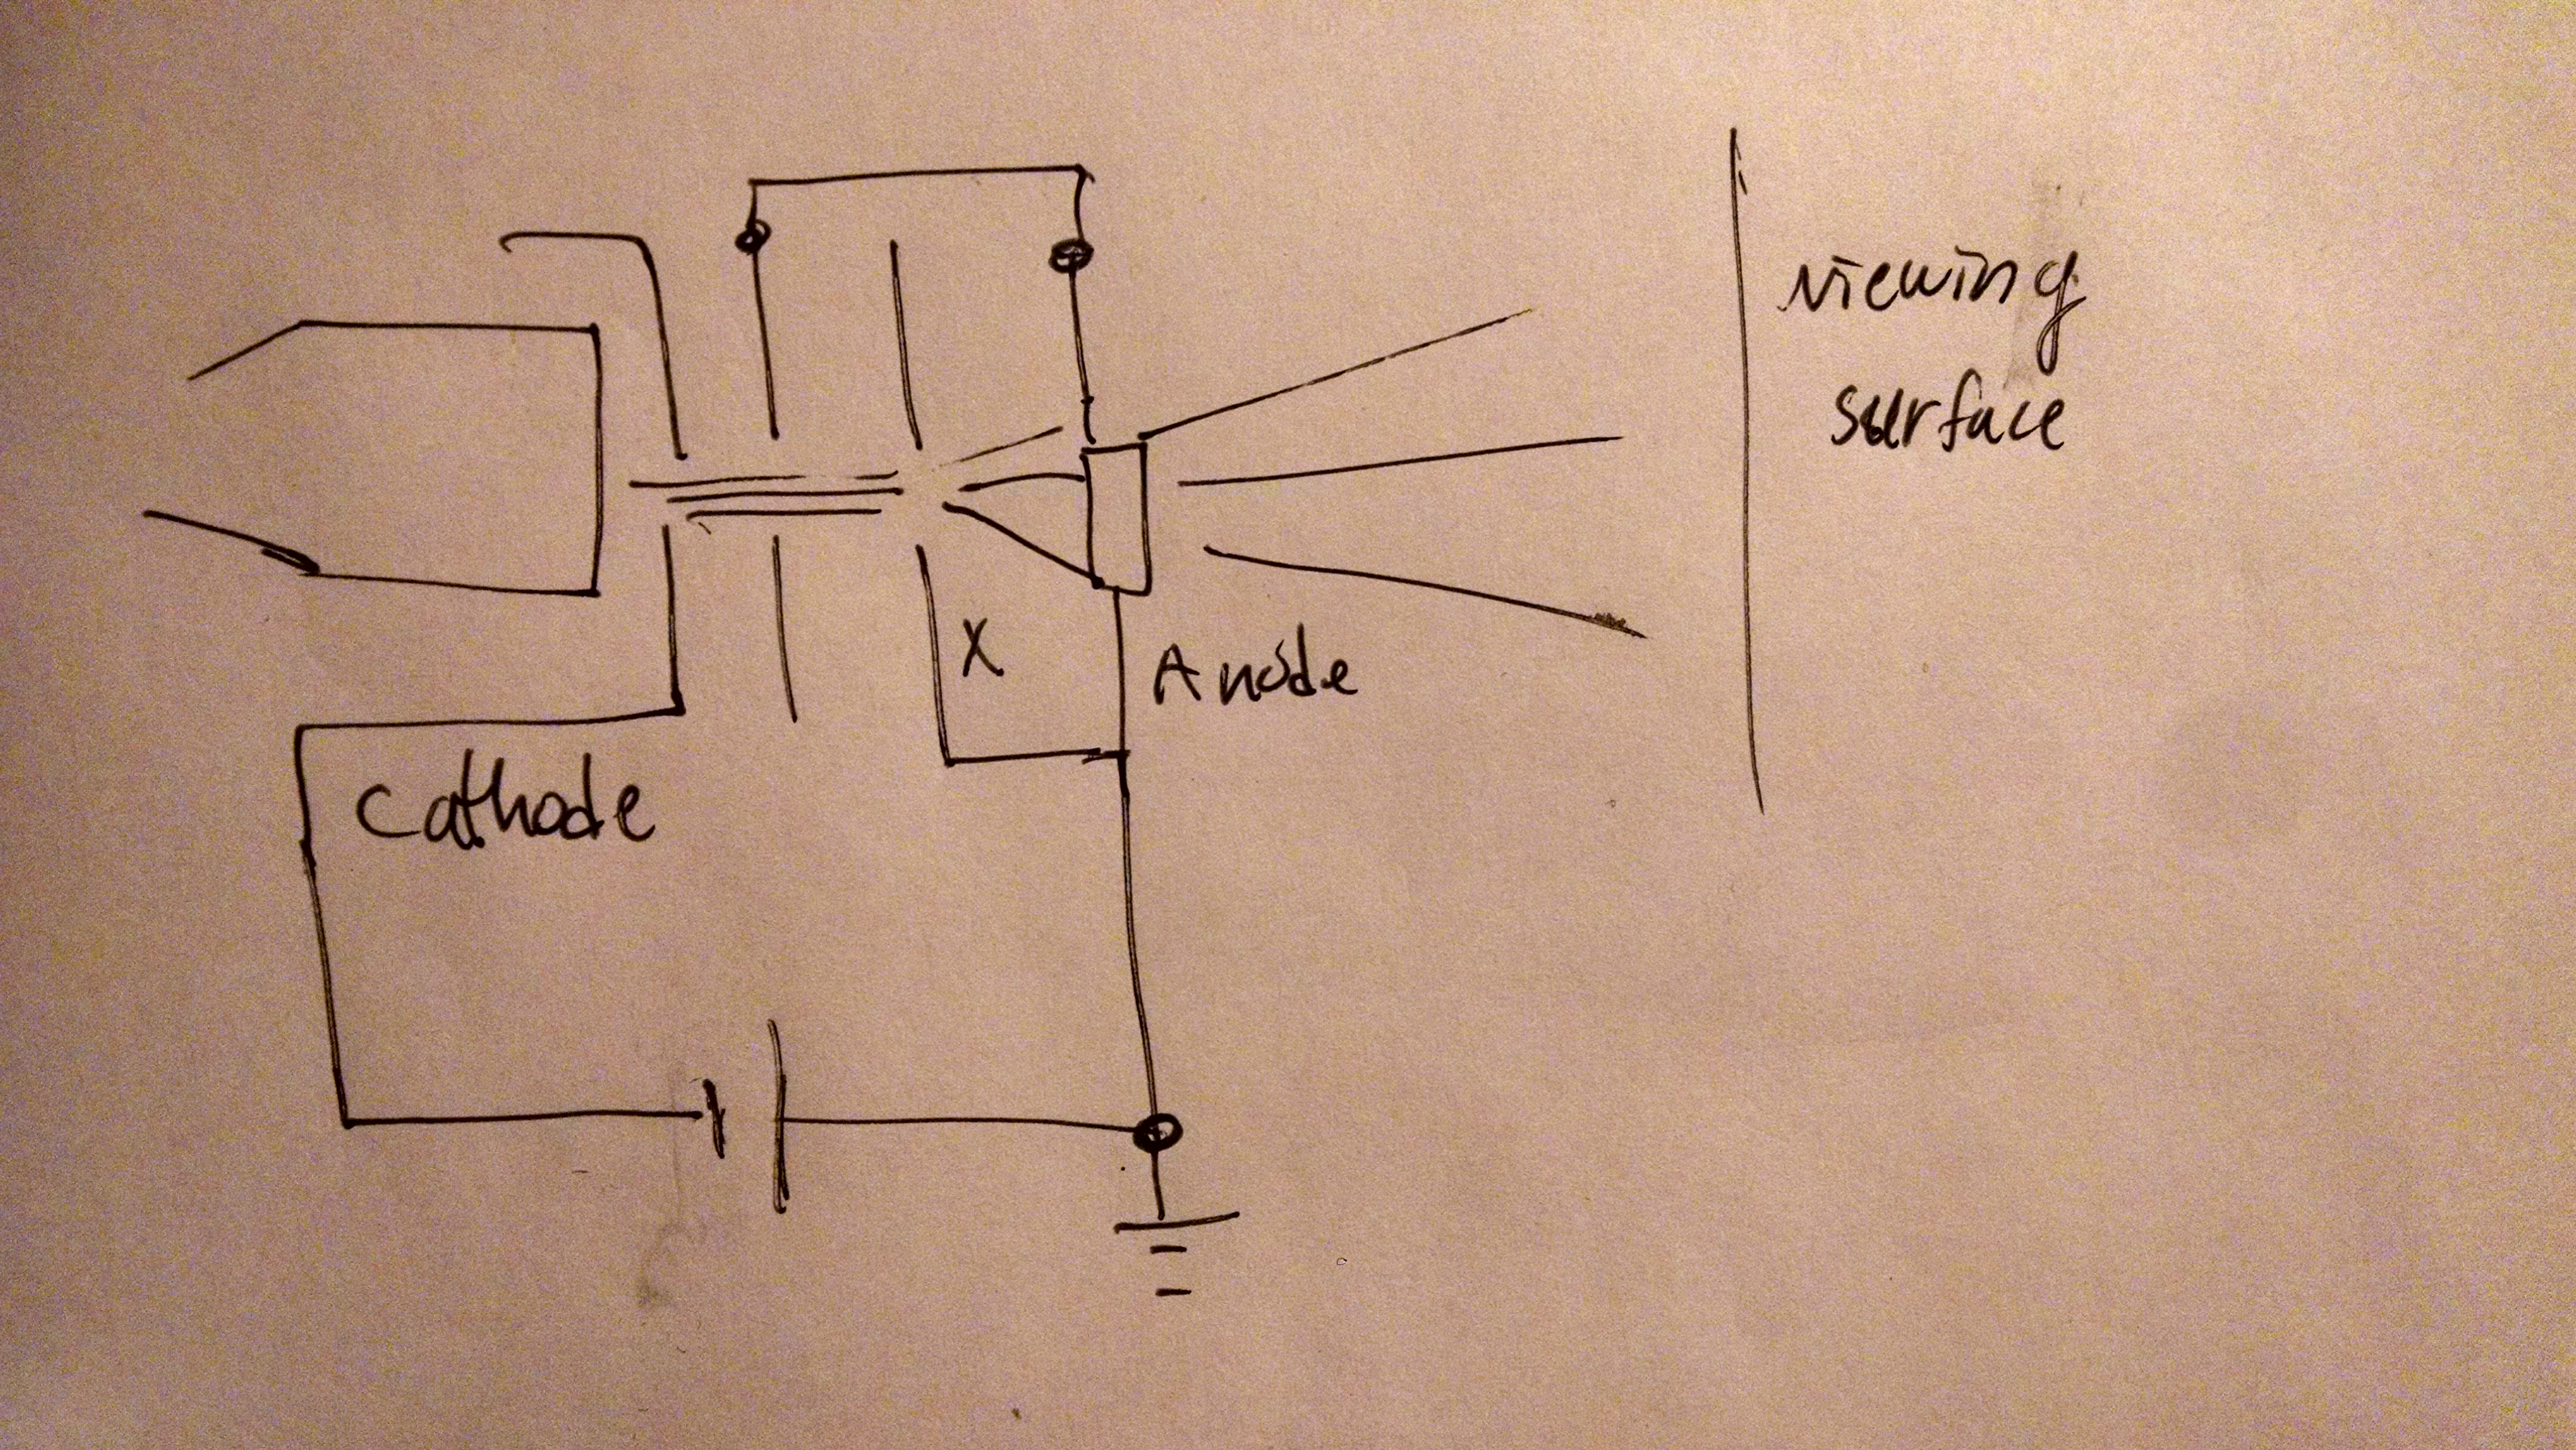
\includegraphics[width=.75\textwidth]{electron_beam2.jpg}
    \label{fig:ebeam2}
\end{figure}


In our second experiment we turned the accelerating voltage from 5.0 kV down to about 3.5 kV and we saw the pattern spread out. This is because the electrons were of lower energy and therefore had less velocity. This decrease in energy corresponds to an increase of wavelength $\lambda$ because we know $ E = hc / \lambda $. So, the pattern spreads out because by Bragg's equation if the wavelength increases and the lattice spacing stays constant then the angle must change. 

In the third part of our experiment we changed the polarity of the focusing electrode from positive to negative. This changes our electron beam from a focused beam to a divergent beam. This result is known from classical optics as the difference between a convergent and divergent lens. In parts 1 and 2 we have a convergent lens that gets focused to the graphite sample, whereas in this part we have a divergent lens that scatters the electrons everywhere. This illuminates the piece of graphite. So, in picture figure \ref{fig:graphite_sample} the bright spots are where there is no or hardly any sample and the dark spots are where there is a lot of the graphite sample. 

\subsection*{Additional Questions from Handout}

Note: in the handout wavelengths are given with the peculiar unit of "C". We believe this is a typo and will therefore assume that this meant to be {\AA}ngstr\"{o}m ({\AA}) 
\medskip

\noindent\textbf{6a.} We are given Bragg's equation and a wavelength of 1.5420 {\AA}, that is first order (n = 1) and that the reflection angle is 21.01 \degree. We can rearrange Bragg's equation to solve for the lattice spacing $d$ 
$$ 
d = \frac{n \lambda}{2 \sin \theta}
$$
If we plug our numbers in (and convert to MKS units of course). We end up with a lattice spacing of 6.408 \e{-11} m. 

\medskip

\noindent \textbf{6b.} We are given that a beam of electrons with energy of 54 ev was directed at a nickel crystal with a lattice spacing of 2.15 {\AA} and an angle of 50\degree. If we plug these values into equation 7 from the handout (making sure to neglect the factor of 2!) we get 1.65 \e{-10} m. 

If we calculate the wavelength using de Broglie's equation. We first find the velocity by setting $54 ev = 1/2 m v ^2 $ and solving for the velocity. We found this to be: 4.36\e{6} m/s. We then plugged that into de Broglie's equation to find the wavelength of 
1.67 \e{-10} m. We conclude that the theoretical value is only off by 0.02\e{-10} m. So, this is a very good experimental result! 
\medskip 

\noindent \textbf{6c.} We are asked to calculate the velocity of neutrons that are scattered with a first-order reflection with $\theta = 30$\degree, a crystal with lattice spacing of d = 1.5 \e{-8} cm and neutrons have mass of 1.66\e{-24} g. We first solve for the wavelength and then we can solve for the velocity using de Broglie's equation. We find the wavelength to be 1.5\e{-10} m. We then solve for the velocity and find it to be 2661 m/s using the equation 
$$ 
v = \frac{h}{m \lambda}
$$

\medskip 

\noindent \textbf{6d.} We are asked to calculate a temperature for part c. We will use the velocity we found of 2661 m/s to find the temperature. We can solve the equation given for temperature. 
$$ 
T = \frac{m v^2}{3 k_B}
$$

where $v$ is the velocity $m$ is the mass of a neutron and $k_B$ is the Boltzmann constant. If we set v = 2661 m/s we find the temperature to be 283.9 K. 






\end{document}